\chapter{Project Planning}
\minitoc
\newpage


\setcounter{secnumdepth}{2} % Resume counting the sections for the toc with a depth of 2 (Sections and sub-sections)
% ----------------------------------- SECTIONS (v) ----------------------------------- %
% ----------------------- DevOps ----------------------- %
\section{Requirements Analysis and Specifications}
The Requirement Specifications provide a comprehensive outline of what the software must do and how it should perform. They are categorized into functional and non-functional requirements. These requirements are informed by the needs of the actors or users of the software, and the desired capabilities of the system.

\subsection{Identification of the Actors}
The iCD toolset web application will cater to a broad range of actors, each with their own specific needs and expectations. These actors can be grouped into three main categories: Companies/Organizations, Individuals, and Educational Institutions.

\begin{itemize}
    \renewcommand\labelitemi{-}
    \item Companies/Organizations include : \\
          \begin{enumerate}
              \item HR Manager : \\
                    They will identify job roles, assess employee skill levels, plan training programs, and evaluate their effectiveness.
              \item Project Managers : \\
                    They will identify skill sets needed for projects, assemble teams based on these skills, assess team members' skills, and arrange training when necessary.
              \item Internal and Consultant Recruiters : \\
                    They will source candidates with specific skill sets, assess candidate skills during hiring, and align candidate skills with company needs.
              \item IT Department Heads : \\
                    They will identify and evaluate internal tasks, address skill gaps in the IT department, and plan for upskilling, reskilling, and cross-skilling initiatives.
              \item CEOs : \\
                    They will understand IT skill requirements for strategic planning, ensure the alignment of the IT workforce with company goals, and define internal tasks aligning with the company's business.
          \end{enumerate}
          \newpage
    \item Individuals include : \\
          \begin{enumerate}
              \item IT Professionals : \\
                    They will identify relevant skills, assess personal skill levels, identify desired job roles or specializations, create a skill development plan, and track progress and achievements.
              \item Students : \\
                    They will identify relevant skills for IT careers, assess personal skill levels, explore potential IT jobs, and create a skill development plan, and track progress and achievements.
              \item IT Job Seekers : \\
                    They will identify in-demand skills for targeted roles, assess personal skill levels, align skills with job requirements, and create a skill development plan.
          \end{enumerate}
    \item Educational Institutions include : \\
          \begin{enumerate}
              \item Curriculum Developers : \\
                    They will design educational programs for skill enhancement, align curricula with industry needs and trends, and evaluate and improve existing programs. 
              \item Faculty Members : \\
                    They will identify skills to teach, align teaching methodologies with the industry, and participate in development programs. 
              \item Career Counselors : \\
                    They will guide students in selecting IT careers, help students understand skill requirements for different roles, and assist students in creating skill development plans. 
              \item Corporate Trainers : \\
                    They will design and offer tailored training programs, assess and address skill gaps within organizations, and collaborate with companies to ensure training effectiveness.  
              \item Program Evaluators : \\
                    They will measure the skill level of IT engineers before and after participation in educational programs, evaluate and improve educational programs, and provide participants with information on their estimated skill levels.  
          \end{enumerate}
          
\end{itemize}

\subsection{Functional Requirement Analysis}
The functional requirements of our project are directly tied to the needs and expectations of the actors involved. Each actor category (Companies/Organizations, Individuals, and Educational Institutions) has unique functionalities that they expect from the system.
\begin{enumerate}
    \item For Companies/Organizations : \\
          For each role within Companies/Organizations, the system will provide the following functionalities:
          \begin{enumerate}
              \item HR Managers : \\
                    \begin{itemize}
                        \renewcommand\labelitemi{-}
                        \item Functionality to identify job roles and required skill sets.
                        \item  Capability to assess employee skill levels.
                        \item Tools to plan employee training programs.
                        \item Systems to evaluate the effectiveness of training initiatives.
                    \end{itemize}
              \item Project Managers : \\
                    \begin{itemize}
                        \renewcommand\labelitemi{-}
                        \item Functionality to identify the skill sets needed for a project.
                        \item Capability to assemble project teams based on skill requirements.
                        \item Tools to assess team members' skill levels.
                        \item Systems to identify skill gaps and arrange training as needed.
                    \end{itemize}
              \item Internal and Consultant Recruiters : \\
                    \begin{itemize}
                        \renewcommand\labelitemi{-}
                        \item Functionality to source candidates with specific skill sets.
                        \item Capability to assess candidate skill levels during the hiring process.
                        \item Tools to align candidate skills with company needs.
                    \end{itemize}
              \item IT Department Heads : \\
                    \begin{itemize}
                        \renewcommand\labelitemi{-}
                        \item Functionality to identify and evaluate internal tasks.
                        \item Capability to address skill gaps in the IT department.
                        \item Tools to plan for upskilling, reskilling, and cross-skilling initiatives.
                    \end{itemize}
              \item CEOs : \\
                    \begin{itemize}
                        \renewcommand\labelitemi{-}
                        \item Functionality to understand IT skill requirements for strategic planning.
                        \item Capability to ensure alignment of IT workforce with company goals.
                        \item Tools to define internal tasks aligning with the company's business.
                    \end{itemize}
          \end{enumerate}
    \item For Individuals : \\
          For each role within the Individuals category, the system will provide the following functionalities :
          \begin{enumerate}
              \item IT Professionals : \\
                    \begin{itemize}
                        \renewcommand\labelitemi{-}
                        \item Functionality to identify relevant skills and knowledge areas.
                        \item Capability to assess personal skill levels.
                        \item Tools to identify desired job roles or specializations.
                        \item Systems to create a skill development plan.
                        \item Features to track progress and achievements (certifications, examinations).
                    \end{itemize}
              \item Students : \\
                    \begin{itemize}
                        \renewcommand\labelitemi{-}
                        \item Functionality to identify relevant skills for IT careers.
                        \item Capability to assess personal skill levels.
                        \item Tools to explore potential IT jobs and specializations.
                        \item Systems to create a skill development plan.
                        \item Features to track progress and achievements (certifications, examinations).
                    \end{itemize}
                    \newpage      
              \item IT Job Seekers : \\
                    \begin{itemize}
                        \renewcommand\labelitemi{-}
                        \item Functionality to identify in-demand skills for targeted roles.
                        \item Capability to assess personal skill levels.
                        \item Tools to align skills with job requirements.
                        \item Systems to create a skill development plan for increased employability.
                    \end{itemize}
          \end{enumerate}
    \item For Educational Institutions : \\
          For each role within the Educational Institutions category, the system will provide the following functionalities :
          \begin{enumerate}
              \item Curriculum Developers : \\
                    \begin{itemize}
                        \renewcommand\labelitemi{-}
                        \item Functionality to design educational programs for skill enhancement (both for companies/organizations and individuals).
                        \item Capability to align curricula with industry needs and trends.
                        \item Tools to evaluate and improve existing programs.
                    \end{itemize}
              \item Faculty Members : \\
                    \begin{itemize}
                        \renewcommand\labelitemi{-}
                        \item Functionality to identify skills and knowledge areas to teach (for both companies/organizations and individuals).
                        \item Capability to align teaching methodologies with industry requirements.
                        \item Features to participate in professional development programs.
                    \end{itemize}
              \item Career Counselors : \\
                    \begin{itemize}
                        \renewcommand\labelitemi{-}
                        \item Functionality to guide students in selecting IT careers.
                        \item Capability to help students understand skill requirements for different roles.
                        \item Tools to assist students in creating skill development plans.
                    \end{itemize}
                    \newpage
              \item Corporate Trainers : \\
                    \begin{itemize}
                        \renewcommand\labelitemi{-}
                        \item Functionality to design and offer tailored training programs for companies/organizations.
                        \item Capability to assess and address skill gaps within organizations.
                        \item Tools to collaborate with companies/organizations to ensure training effectiveness.
                    \end{itemize}
              \item Program Evaluators : \\
                    \begin{itemize}
                        \renewcommand\labelitemi{-}
                        \item Functionality to measure the skill level of IT engineers before and after participation in educational programs.
                        \item Capability to evaluate and improve educational programs based on skill level assessments.
                        \item Tools to provide participants with information on their estimated skill levels based on program completion, passing certifying examinations, etc.
                    \end{itemize}
          \end{enumerate}
          
\end{enumerate}

%  ----------------------- Non-Functional Requirements ----------------------- %
\subsection{Non-Functional Requirements Analysis}
Non-functional requirements define the system's properties or characteristics, such as performance, security, and usability. They play a crucial role in the system's operation, as they outline the system's behavior. The following are the non-functional requirements for our web application :

\begin{enumerate}
    \item Usability: The system should be user-friendly and intuitive to ensure that all types of users, irrespective of their technical proficiency, can efficiently utilize the application. It should also include a comprehensive help system and user guide.
    \item Performance: The system should be highly responsive and capable of handling multiple simultaneous users without any degradation in performance. It should also be scalable to accommodate an increasing number of users and data over time.
    \item Compatibility: The system should be compatible with various devices, platforms, and browsers to maximize accessibility. It should adhere to responsive design principles for optimal display on different screen sizes and resolutions.
    \item Maintainability: The system should be designed in a modular manner, allowing for easy updates, modifications, and debugging. It should also provide tools for tracking and resolving any issues that may arise.
    \item Interoperability: The system should seamlessly integrate with the iCD toolset and the Airtable database. It should also provide APIs or other means for possible future integrations with other systems.
\end{enumerate}



% ----------------------- Comparative Analysis ----------------------- %
\section{System Overview and Major Use Cases}

\subsection{Global System Use Case Diagram}
\begin{figure}[H]
    \centering
    \makebox[\textwidth]{\includegraphics[width=\linewidth]{src/assets/images/Companies-use-cases.jpg}}
    \caption{ Global System Use-Case Diagram }
    \label{fig:Global_System_UseCase_Diagram}
\end{figure}

\subsection*{Description}
This diagram provides an overall view of the entire system, encompassing all functionalities and interactions between various user roles and the system. It represents all the major use cases and offers a comprehensive understanding of the system's purpose and the problems it aims to solve.

\subsection{Job Description Definition Use-Case Diagram}
\begin{figure}[H]
    \centering
    \makebox[\textwidth]{\includegraphics[width=0.9\linewidth]{src/assets/images/HRM-Global-Use-Case.jpg}}
    \caption{ Global System Use-Case Diagram }
    \label{fig:Job_Description_Definition_UseCase_Diagram}
\end{figure}

\subsection*{Description}
This diagram focuses on one specific use case - the job description definition. It highlights the flow of interactions involved in defining a job description, demonstrating how various user roles contribute to this process over the course of the project's three sprints. This focused view helps illuminate the intricate details of this complex use case, shedding light on its importance and relevance within the broader context of the system. It complements the global system use case diagram by delving deeper into one of the system's key functionalities.

\section{Project management with Scrum}
\subsection{Team and roles}
In this sub-section, we present the actors involved in the different phases of our project and the preparation of this report. Our development team consists of two individuals responsible for the project realization, from design to development. The Product Owner, who represents the stakeholders, defines the needs, priorities, and functionalities, guiding the development team's activities. The Scrum Master is the orchestrator, ensuring smooth project execution and fostering a positive team atmosphere.

\begin{table}[H]
    \renewcommand{\arraystretch}{1.5}%
    \caption{Scrum Team Roles and Actors}
    \centering
    \medskip
    \begin{tabularx}{\textwidth} {
            | >{\hsize=0.5\hsize\raggedright\arraybackslash}X
            | >{\hsize=1.5\hsize\raggedright\arraybackslash}X |}
        \hline
        \rowcolor{primary} \textbf {Role} & \textbf {Actor}                    \\
        \hline
        Scrum Team                        & Jamil Ben Brahim, Ahmed Amine Hlel \\
        \hline
        Product Owner                     & Adrien L. Beaulieu                 \\
        \hline
        Scrum Master                      & Adrien L. Beaulieu                 \\
        \hline
    \end{tabularx}
\end{table}

\subsection{General Product Backlog}
The Backlog is a crucial artifact in Scrum, encompassing the functional or technical characteristics that make up the desired product. In the subsequent sections, we present a general backlog for our product, followed by a more detailed backlog for the HR Manager persona, the main focus of our work so far.


\begin{table}[H]
    \renewcommand{\arraystretch}{1.5}%
    \caption{Product Backlog}
    \centering
    \medskip
    \small
    \begin{tabularx}{\textwidth} {
            | >{\hsize=1\hsize\raggedright\arraybackslash}X
            | >{\hsize=0.5\hsize\raggedright\arraybackslash}X
            | >{\hsize=2\hsize\raggedright\arraybackslash}X
            | >{\hsize=0.5\hsize\raggedright\arraybackslash}X |}
        \hline
        \rowcolor{primary} \textbf {Epic/Feature}             & \textbf {Persona} & \textbf {User Story}                                                                                                           & \textbf {Priority} \\
        \hline
        System Access/Account Management                      & HR Manager        & As an HR Manager, I want to sign up, create my profile, and login to access the system                                         & High               \\
        \hline
        User Profile Management/Profile Update                & HR Manager        & As an HR Manager, I want to update my profile information and delete the account if necessary                                  & High               \\
        \hline
        Job Description Definition/Job Selection              & HR Manager        & As an HR Manager, I want to select a job description and the associated specialized field to define roles and responsibilities & High               \\
        \hline
        Job Description Definition/Skill Selection            & HR Manager        & As an HR Manager, I want to filter and select the necessary skills for the chosen job description                              & High               \\
        \hline
        Job Description Definition/Task Selection             & HR Manager        & As an HR Manager, I want to fetch and select the tasks related to the chosen skills                                            & High               \\
        \hline
        Job Description Definition/Job Description Generation & HR Manager        & As an HR Manager, I want to generate the job description using the selected skills and tasks                                   & High               \\
        \hline
        Advanced Features/Email Job Description               & HR Manager        & As an HR Manager, I want to email the generated job description to potential candidates directly from the system               & Medium             \\
        \hline
        Advanced Features/Print to PDF                        & HR Manager        & As an HR Manager, I want to print the nested skills and tasks to a PDF format for documentation or offline use                 & Medium             \\
        \hline
        Advanced Features/Chatbot Interaction                 & HR Manager        & As an HR Manager, I want to interact with a chatbot to understand the system better and get guidance on the process            & Medium             \\
        \hline
    \end{tabularx}
    \normalsize
\end{table}

\subsection*{Scope of work :}
In the context of this project and given the timeline constraints, we specifically focused on developing and implementing user stories associated with the HR Manager persona from the Companies/Organizations category.

\subsection{Sprints Planning}
\begin{enumerate}
    \item Study and realization of the Sprint 1 : \\
          Sprint 1: System Access and User Profile Management
          \begin{itemize}
              \renewcommand\labelitemi{-}
              \item User Story 1: As an HR Manager, I want to sign up and create my profile so that I can access the system. \\
                    \begin{itemize}
                        \item Subtask 1.1: Design and implement the signup process
                        \item Subtask 1.2: Design and implement the profile creation process
                    \end{itemize}
              \item User Story 2: As an HR Manager, I want to login into the system so that I can access the features. \\
                    \begin{itemize}
                        \item Subtask 2.1: Design and implement the login process
                    \end{itemize}
              \item User Story 3: As an HR Manager, I want to be able to update my profile information in the account settings and delete the account. \\
                    \begin{itemize}
                        \item Subtask 3.1: Develop a feature that allows HR Managers to update their profile information or delete the account.
                        \item Subtask 3.2: Integrate this feature into the system.
                    \end{itemize}
          \end{itemize}
          
    \item Study and realization of the Sprint 2 : \\
          Sprint 2: Job Description Definition
          \begin{itemize}
              \renewcommand\labelitemi{-}
              \item User Story 1: As an HR Manager, I want to select a job description and the associated specialized field so that I can define roles and responsibilities. \\
                    \begin{itemize}
                        \item Subtask 1.1: Implement a dropdown feature for HR Managers to select a job description and specialized field
                        \item Subtask 1.2: Connect the dropdown selections to the Airtable database to fetch relevant data
                    \end{itemize}
              \item User Story 2: As an HR Manager, I want to filter and select the necessary skills for the chosen job description so that I can ensure the necessary competencies for the job are outlined. \\
                    \begin{itemize}
                        \item Subtask 2.1: Implement a feature that fetches skills related to the selected job description from the Airtable database
                        \item Subtask 2.2: Utilize Algolia search engine capabilities to enable HR Managers to filter and search through the skills
                    \end{itemize}
              \item User Story 3: As an HR Manager, I want to fetch and select the tasks related to the chosen skills so that I can ensure all necessary tasks for the job are included. \\
                    \begin{itemize}
                        \item Subtask 3.1: Implement a feature that fetches tasks related to the selected skills from the Airtable database
                        \item Subtask 3.2: Utilize Algolia search engine capabilities to enable HR Managers to filter and search through the tasks
                    \end{itemize}
              \item User Story 4: As an HR Manager, I want to generate the job description using the selected skills and tasks so that I can have a comprehensive job description. \\
                    \begin{itemize}
                        \item Subtask 4.1: Implement a feature that generates a job description using the GPT-3 API based on the selected skills and tasks
                        \item Subtask 4.2: Display the generated job description for the HR Manager
                        \item Subtask 4.3: Implement features for HR Managers to delete or update the generated job description
                    \end{itemize}
          \end{itemize}
          
    \item Study and realization of the Sprint 3 : \\
          Sprint 3: Advanced Features and Finishing Touches
          \begin{itemize}
              \renewcommand\labelitemi{-}
              \item User Story 1: As an HR Manager, I want to email the generated job description to potential candidates directly from the system.\\
                    \begin{itemize}
                        \item Subtask 1.1: Develop a process to email job descriptions
                        \item Subtask 1.2: Implement the process in the system
                    \end{itemize}
              \item User Story 2: As an HR Manager, I want to print the nested skills and tasks to a PDF format for documentation or offline use. \\
                    \begin{itemize}
                        \item Subtask 2.1: Develop a process to convert selected skills and tasks to a PDF
                        \item Subtask 2.2: Implement the process in the system
                    \end{itemize}
              \item User Story 3: As an HR Manager, I want to interact with a chatbot to understand the system better and get guidance on the process. \\
                    \begin{itemize}
                        \item Subtask 3.1: Develop a chatbot using GPT-3
                        \item Subtask 3.2: Integrate the chatbot into the system 
                    \end{itemize}
          \end{itemize}
\end{enumerate} 

\vspace{2cm}

\begin{figure}[H]
    \centering
    \makebox[\textwidth]{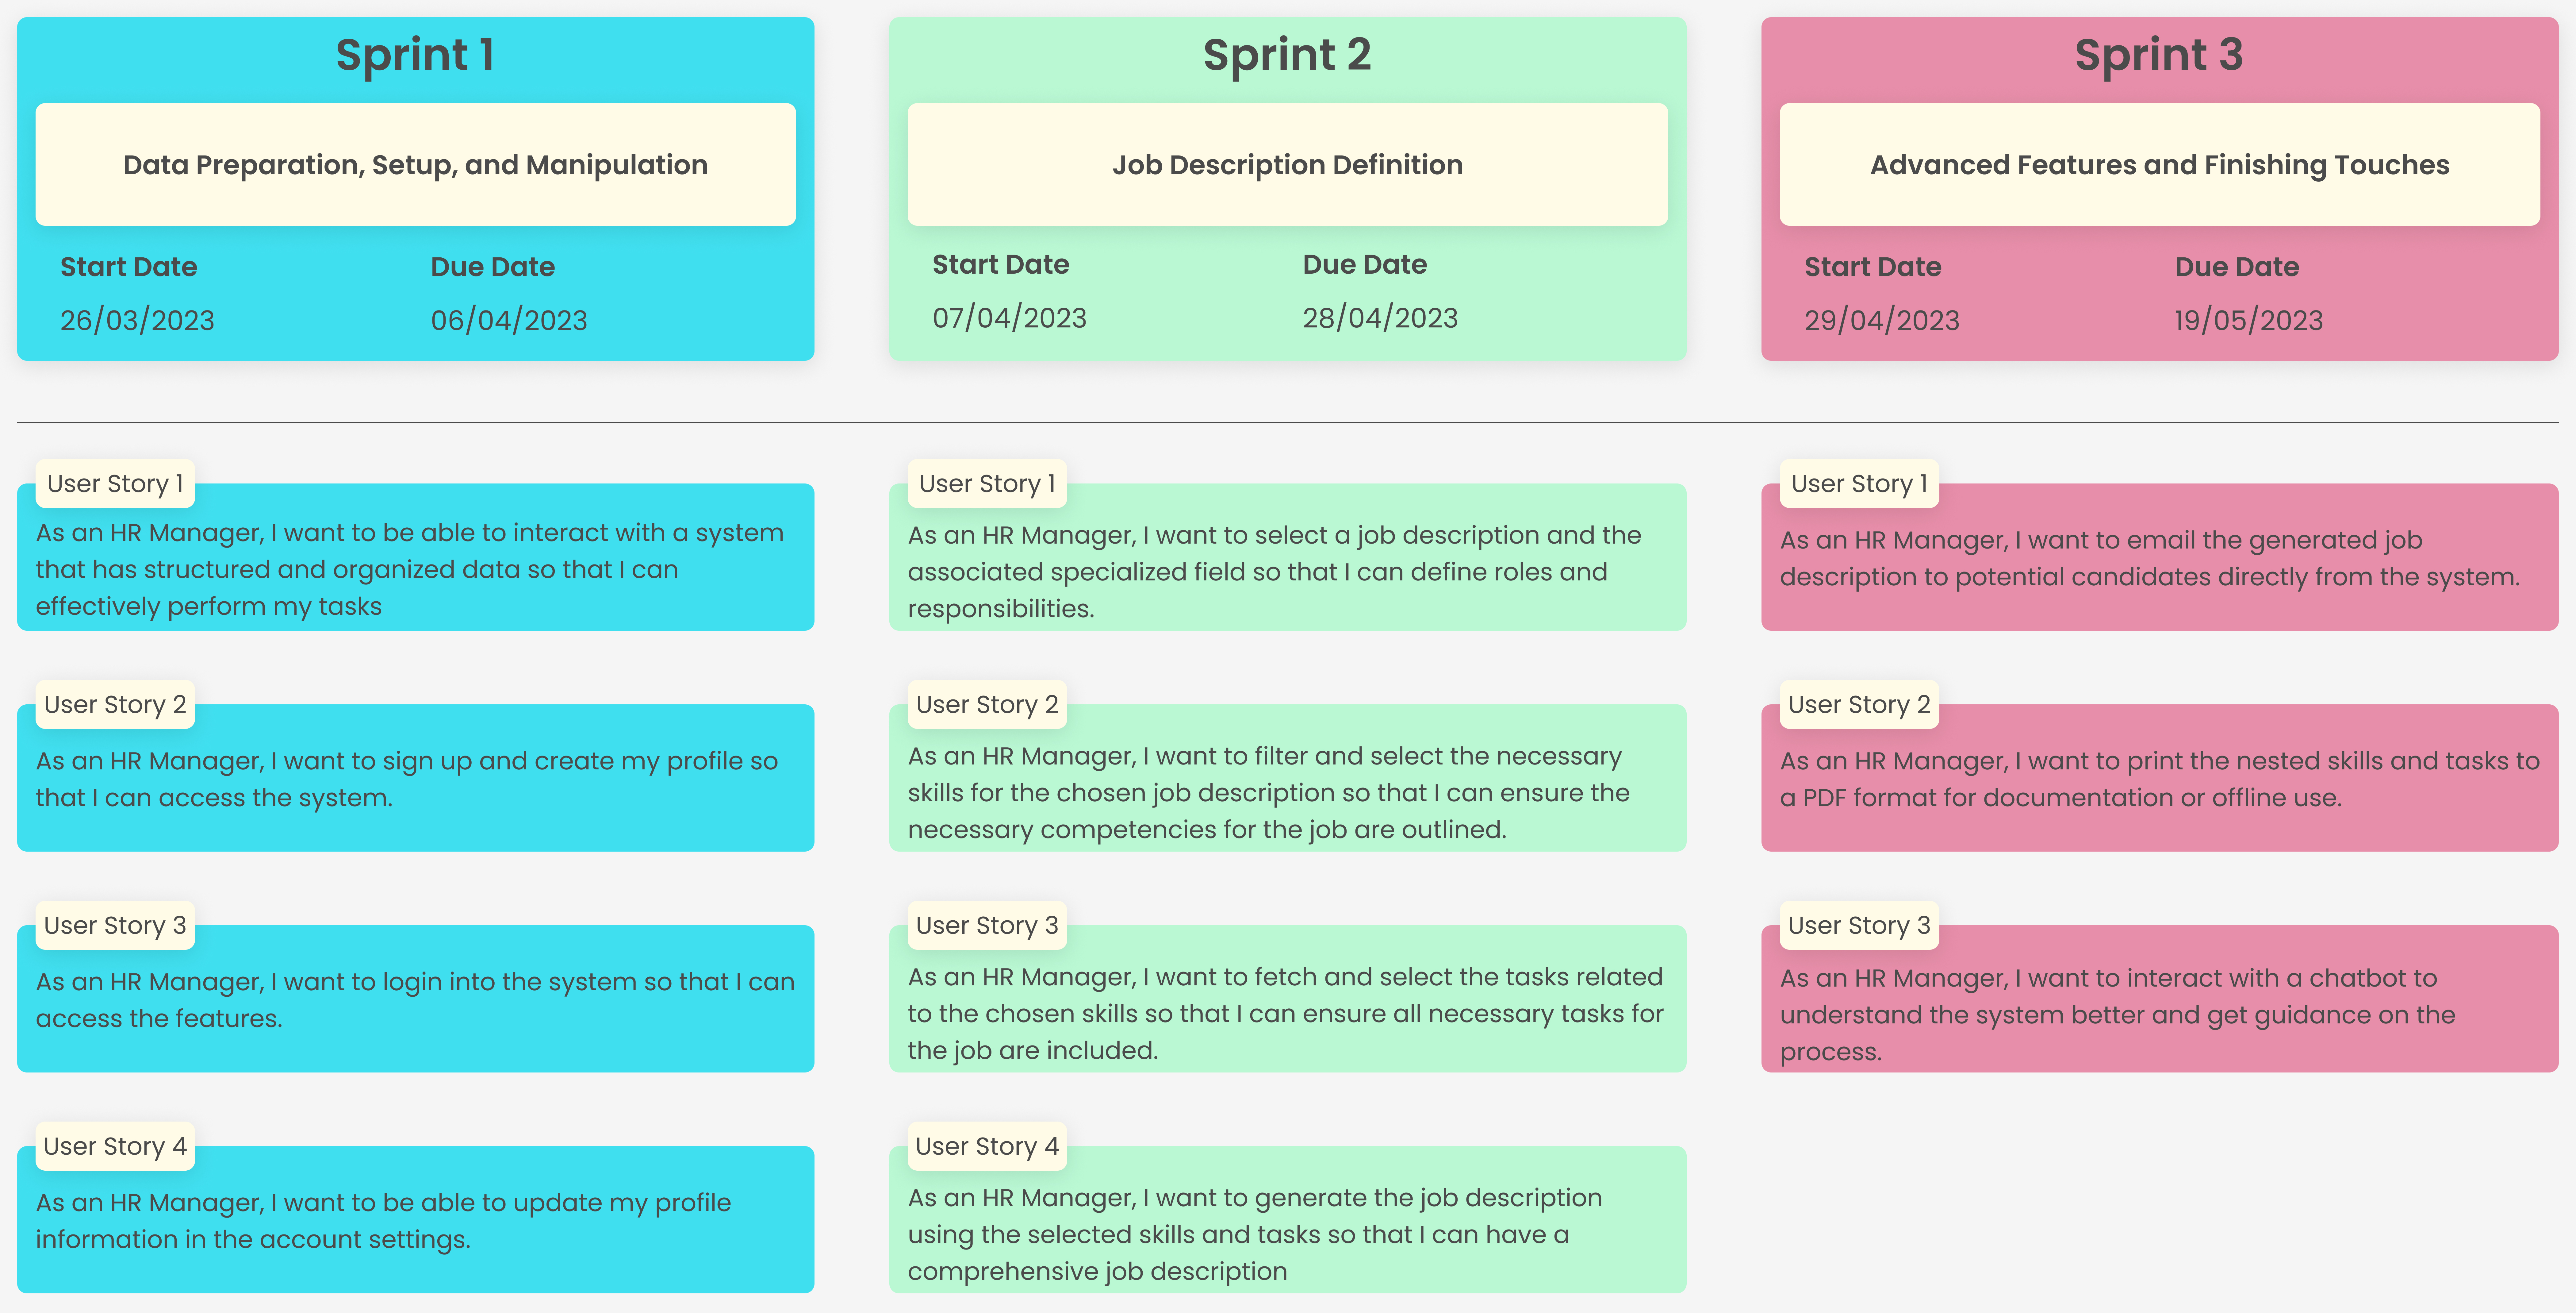
\includegraphics[width=1.25\linewidth]{src/assets/images/Sprints.jpg}}
    \caption{ Sprints Planning Diagram }
    \label{fig:Sprints_Graph}
\end{figure}

\newpage
\subsection{interface mockups}
In this section, we will present the interface mockups for our project. These mockups provide a visual representation of the user interface (UI) that we have designed for our application. They serve as a blueprint for the layout and functionality of the application, illustrating how users, particularly HR managers, will interact with the system. The interface mockups were created with a focus on user-friendliness and intuitive navigation, ensuring that HR managers can easily utilize the IT Competency Dictionary (iCD) toolset through our application. From account creation and management to job description definition and advanced features, these mockups encapsulate the entire user journey within our application.

\begin{figure}[H]
    \centering
    \makebox[\textwidth]{\includegraphics[width=\linewidth]{src/assets/mockups/Login-Page.jpg}}
    \caption{ Sign-In Interface Mockup }
    \label{fig:Sign-In-Interface-Mockup}
\end{figure}

\begin{figure}[H]
    \centering
    \makebox[\textwidth]{\includegraphics[width=\linewidth]{src/assets/mockups/Register-Page.jpg}}
    \caption{ Sign-Up Interface Mockup }
    \label{fig:Sign-Up-Interface-Mockup}
\end{figure}

\begin{figure}[H]
    \centering
    \makebox[\textwidth]{\includegraphics[width=\linewidth]{src/assets/mockups/Profile-Page-1.jpg}}
    \caption{ First Profile Page Interface Mockup }
    \label{fig:First-Profile-Page-Interface-Mockup}
\end{figure}

\begin{figure}[H]
    \centering
    \makebox[\textwidth]{\includegraphics[width=\linewidth]{src/assets/mockups/Profile-Page-2.jpg}}
    \caption{ Second Profile Page Interface Mockup }
    \label{fig:Second-Profile-Page-Interface-Mockup}
\end{figure}

\begin{figure}[H]
    \centering
    \makebox[\textwidth]{\includegraphics[width=\linewidth]{src/assets/mockups/Account-Settings-1.jpg}}
    \caption{ Account Settings Page Interface Mockup }
    \label{fig:Account-Settings-Page-Interface-Mockup}
\end{figure}

\begin{figure}[H]
    \centering
    \makebox[\textwidth]{\includegraphics[width=\linewidth]{src/assets/mockups/Use-case-1-1.jpg}}
    \caption{ Job Description Definition Main Page Interface Mockup }
    \label{fig:Job-Description-Definition-Main-Page-Interface-Mockup}
\end{figure}


\begin{figure}[H]
    \centering
    \makebox[\textwidth]{\includegraphics[width=\linewidth]{src/assets/mockups/Use-case-1-2.jpg}}
    \caption{ Dropdown Selection Page Interface Mockup }
    \label{fig:Dropdown-Selection-Page-Interface-Mockup}
\end{figure}


\begin{figure}[H]
    \centering
    \makebox[\textwidth]{\includegraphics[width=\linewidth]{src/assets/mockups/Dashboard-1-1.jpg}}
    \caption{ User Dashboard Page Interface Mockup }
    \label{fig:User-Dashboard-Page-Interface-Mockup}
\end{figure}


\begin{figure}[H]
    \centering
    \makebox[\textwidth]{\includegraphics[width=\linewidth]{src/assets/mockups/Use-case-1-3.jpg}}
    \caption{ Skill Selection Page Interface Mockup }
    \label{fig:Skill-Selection-Page-Interface-Mockup}
\end{figure}



\newpage
\section{Working Environment}
This part is reserved for the presentation of all of the hardware and software used in the realization of the project and includes but is not limited to; programming languages, frameworks, technologies, etc...
\subsection{Hardware Environment}
The hardware environment for the development and testing of the application consists of two main systems with the following specifications:

\begin{enumerate}
    \item MSI gp76 leopard :
          \begin{itemize}
              \item Graphics: RTX 3060
              \item Processor: Intel Core i7 10th Gen
              \item Memory: 16 GB RAM
              \item Storage: 1 TB SSD
              \item Operating System: Windows 10 Home Single Language
          \end{itemize}
    \item Dell G3 1500 :
          \begin{itemize}
              \item Graphics: GTX 1650
              \item  Processor: Intel Core i5 10th Gen
              \item Memory: 8 GB RAM
              \item Storage: 1 TB HDD, 256 GB SSD
              \item Operating System: Windows 10 Pro
          \end{itemize}
\end{enumerate}

\subsection{Software Environment}
The software environment used for the development of the application includes a combination of code editing, API testing, and design tools:

\begin{itemize}
    \renewcommand\labelitemi{-}
    \item Code Editing: Visual Studio Code is used as the primary code editor for writing and debugging the code for the back-end.
    \item API Testing: Postman and Amnesia are used for testing APIs and checking database interactions.
    \item Design: Figma is used for designing the user interface and user experience of the application.
\end{itemize}

\subsection{ Application Program Interface (API) Choice}
The application interacts with several APIs for data handling and advanced functionality:
\begin{itemize}
    \renewcommand\labelitemi{-}
    \item Render APIs: These are used to interact with the back-end services hosted on the Render cloud application hosting platform.
    \item Algolia APIs: These are used to create an index of all skill items in the iCD toolset and provide search capabilities in the application.
    \item GPT-3.5 Turbo API: This API from OpenAI is used to generate job descriptions based on the selected skills and tasks.
\end{itemize}

\subsection{Front-End Technology Choice}
The team chose {\color{purple} FlutterFlow} as the front-end development platform for the application. FlutterFlow is a revolutionary low-code platform that allows developers to design, build and prototype applications rapidly. It provides a visually intuitive interface that enables the building and testing of the UI in real-time. This significantly reduces the time and effort required for UI development and allows the team to focus more on the functionality and user experience of the application.

\begin{figure}[H]
    \centering
    \makebox[\textwidth]{\includegraphics[width=\linewidth]{src/assets/logos/flutterflowLogo.png}}
    \caption{  Logo Of FlutterFlow }
    \label{fig:FlutterFlow_Logo}
\end{figure}

% \newpage
FlutterFlow also supports custom code in {\color{purple} Dart}, which is a client-optimized language for fast apps on any platform. Dart was used extensively in this project to implement custom widgets, functions, and actions to meet the specific needs of the application. The language's robust library and powerful features facilitated the development of interactive features in the application, such as dropdowns for job descriptions, the Algolia search function for skill selection, and the chatbot for user assistance.

\begin{figure}[H]
    \centering
    \makebox[\textwidth]{\includegraphics[width=0.8\linewidth]{src/assets/logos/dartLogo.png}}
    \caption{  Logo Of Dart }
    \label{fig: Dart_Logo}
\end{figure}

\subsection{Back-End Technology Choice}
The back-end of the application was developed using {\color{purple}JavaScript} with the {\color{purple}Express.js} framework. JavaScript is a high-level, interpreted scripting language that conforms to the ECMAScript specification. It's widely used for creating and controlling web pages, making it a fundamental technology for web development.

\begin{figure}[H]
    \centering
    \makebox[\textwidth]{\includegraphics[width=0.5\linewidth]{src/assets/logos/js Logo.png}}
    \caption{  Logo Of JavaScript }
    \label{fig: JS_Logo}
\end{figure}

Express.js is a fast, unopinionated, and minimalist web framework for Node.js. It's designed for building web applications and APIs. In this project, Express.js was used to structure the data from the iCD toolset and handle API routes, ensuring efficient and reliable data management.

\begin{figure}[H]
    \centering
    \makebox[\textwidth]{\includegraphics[width=0.8\linewidth]{src/assets/logos/expressJsLogo.png}}
    \caption{  Logo Of ExpressJs }
    \label{fig: ExpressJS_Logo}
\end{figure}

For database management, we used  {\color{purple}Airtable} and  {\color{purple}Firebase}. Airtable is a cloud-based software company that blends a traditional spreadsheet with a database. It offers a variety of views to work with data, including grid, calendar, kanban, gallery, and form. 

\begin{figure}[H]
    \centering
    \makebox[\textwidth]{\includegraphics[width=0.8\linewidth]{src/assets/logos/airtableLogo.png}}
    \caption{  Logo Of Airtable }
    \label{fig: Airtable_Logo}
\end{figure}

\newpage
Firebase Firestore is a flexible, scalable database for mobile, web, and server development from Firebase and Google Cloud. It keeps data in sync across client apps through real-time listeners and offers offline support for mobile and web, making it an excellent choice for handling user information and authentication.

\vspace{2cm}

\begin{figure}[H]
    \centering
    \makebox[\textwidth]{\includegraphics[width=0.8\linewidth]{src/assets/logos/firebaseLogo.png}}
    \caption{  Logo Of Firebase }
    \label{fig: Firebase_Logo}
\end{figure}

We used {\color{purple}Render}, a unified platform to build and run all applications and websites, for hosting the web services. Render makes it easier to manage and scale apps with fully managed PostgreSQL, Redis, cron jobs, background workers, and more, all on a unified platform.

\begin{figure}[H]
    \centering
    \makebox[\textwidth]{\includegraphics[width=0.8\linewidth]{src/assets/logos/rederLogo.png}}
    \caption{  Logo Of Render }
    \label{fig: Render_Logo}
\end{figure}


\newpage
{\color{purple}Algolia} was used to enhance the application's search capabilities. Algolia is a powerful and flexible search and discovery API that delivers real-time results from the first keystroke. Its powerful features enabled the application to handle the extensive data from the iCD toolset and provide a user-friendly experience.

\begin{figure}[H]
    \centering
    \makebox[\textwidth]{\includegraphics[width=0.8\linewidth]{src/assets/logos/algoliaLogo.png}}
    \caption{  Logo Of Algolia }
    \label{fig: Algolia_Logo}
\end{figure}


For the automated generation of job descriptions and for the interactive chatbot feature, the team utilized the {\color{purple}GPT-3.5 Turbo API} from OpenAI. The GPT API provides a general-purpose "text in, text out" interface, making it easy to apply the capabilities of the models to a wide range of tasks. The use of system context related to the iCD toolset ensured that the chatbot provided related and helpful information to the users.

\begin{figure}[H]
    \centering
    \makebox[\textwidth]{\includegraphics[width=0.4\linewidth]{src/assets/logos/openAILogo.png}}
    \caption{  Logo Of OpenAI }
    \label{fig: OpenAI_Logo}
\end{figure}

With these technologies combined, We were able to build an efficient and user-friendly application that simplifies the use of the iCD toolset.


\section{Proposed architecture}
\subsection{General Presentation of the Proposed Solution}

% The proposed solution is a web application designed to simplify the usage of the iCD toolset, which is a comprehensive set of task and skill dictionaries. The iCD toolset comes in its raw form as Excel files and graphs, making it challenging to interact with and extract relevant information. Our web application addresses this challenge by importing, filtering, and structuring the iCD toolset data into a user-friendly format.

% The primary users we focused on for the sake of this application MVP (Minimum Viable Product) are Human Resource Managers, who use the application to define job descriptions. These users can select a job from a series of dropdown menus, and the application will display the skills required for the selected job. Users can then filter and search for the desired skills using the Algolia search engine, which we have integrated into our application. After the skills are selected, the application fetches and displays the tasks related to those skills. Users can then generate a job description, which is created using the GPT-3.5 Turbo model from OpenAI. All generated job descriptions are stored in a Firestore database and can be updated or deleted as required.

% In addition to these features, the application includes a chatbot that uses the GPT-API to provide context-specific information about the iCD toolset to the users.

Our web application simplifies the iCD toolset, originally in Excel files and graphs, by making the data user-friendly. The MVP focuses on Human Resource Managers, enabling them to define job descriptions. Users can select jobs from dropdown menus, view required skills, and use the Algolia search engine for skill filtering. The application shows tasks related to selected skills and generates job descriptions via the GPT-3.5 Turbo model from OpenAI. Generated descriptions are stored in a Firestore database for updating or deletion. A GPT-API-powered chatbot is included for context-specific iCD toolset information.


\subsection{General Architecture}

The application's architecture is designed with a focus on simplifying the interaction between the user and the iCD toolset data. It consists of several key components:

\begin{itemize}
    \item Front-End: Built with FlutterFlow, our front-end enables HR managers to select jobs, view, filter, and search skills, choose related tasks, and generate job descriptions.
    \item Back-End: Leveraging JavaScript and Express.js, our back-end structures the raw iCD data and exposes it via APIs hosted on Render.
    \item Database: The application uses two databases: Airtable and Firestore. The iCD toolset data is imported and filtered into an Airtable database, while Firestore is used to store user information and generated job descriptions.
    \item Third-Party Services: The application uses several third-party services. Algolia is used to create an index of all skill items and task items and provide search capabilities. The GPT-3.5 Turbo model from OpenAI is used to generate job descriptions. Firebase is used for user authentication and data storage.
    \item Chatbot: A chatbot is included in the application to provide users with context-specific information about the iCD toolset. The chatbot also uses the GPT-API from OpenAI and is designed to provide suggestions that are updated based on the user's interactions with the application.
\end{itemize}



\begin{landscape}
    \begin{figure*}
        \centering
        \includegraphics[width=0.95\linewidth]{src/assets/images/ICD-Application-Global-Architecture-Final-Edition.jpg}
        \caption{Application General Architecture}
        \label{fig:GeneralArchitecture}
    \end{figure*}
\end{landscape}



\section{Data Preparation, Setup, and Manipulation}
% The primary aim of the project was to design and implement a system that enables {\color{newBlue}\textbf{HR}} managers to effectively define job roles and responsibilities using the IT Competency Dictionary (iCD). 
% The iCD, a comprehensive toolset developed in Japan, consists of a {\color{darkPurple}\textbf{Task Dictionary}} outlining specific IT business tasks and a {\color{darkgreen}\textbf{Skill Dictionary}} detailing the necessary IT skills required to perform these tasks. 
% This toolset, originally provided in Excel format, contains essential elements from three previous skill standards in Japan, making it a comprehensive resource for defining IT job roles and responsibilities.
The project's primary goal was to create a system that allows {\color{newBlue}\textbf{HR}} managers to effectively define job roles using the IT Competency Dictionary (iCD). The iCD, a comprehensive toolset from Japan, includes a {\color{darkPurple}\textbf{Task Dictionary}} and a {\color{darkgreen}\textbf{Skill Dictionary}}. Originally in Excel format, the iCD integrates elements from three previous Japanese skill standards, making it a valuable resource for defining IT roles.


\begin{itemize}
    \item Task 1: \\
          Import the raw ICD toolset data into the Airtable database with necessary modifications.
    \item Task 2: \\
          Create and deploy a web server that fetches and structures the data from the Airtable database.
    \item Task 3: \\
          Integrate the web server into the FlutterFlow application to use the structured data.
    \item Task 4: \\
          Develop and implement functions and actions to display and manipulate the data as required for the specific use case.
\end{itemize}


\subsection{Data Setup}

To effectively utilize the iCD toolset, the first step was to import the raw data into {\color{limeGreen}\textbf{Airtable}}, a cloud-based database management system. 
This required converting the Excel-based iCD toolset into a format compatible with Airtable. 
During this process, the data was also meticulously cleaned and reorganized to suit the project's specific requirements. \\
$ \rightarrow $ \quad For instance, duplicate entries were removed, errors in the data were corrected, and data fields were restructured to optimize retrieval and analysis in later stages of the project.

\subsection{Web Service}

Following the successful import of data into Airtable, a {\color{limeGreen}\textbf{web service}} was developed to interact with this data. 
This service, designed using Node.js (or another suitable technology), was tasked with fetching data from Airtable and structuring it in a way that would facilitate easy manipulation and display on the front-end application. 
This involved processes such as validation of the fetched data, as well as sorting and filtering to ensure the most relevant data was sent to the front-end. 
Once developed, this service was deployed on Render, making it accessible for use by the FlutterFlow application.


\subsection{FlutterFlow Integration}
After deploying the web server, it was integrated into the {\color{limeGreen}\textbf{FlutterFlow application}}. 
This entailed establishing a reliable connection between the server and the application, and ensuring that the application could send requests to, and receive responses from, the server correctly. 
A vital part of this integration was to ensure the structured data provided by the server was correctly handled and displayed within the FlutterFlow application, allowing for a seamless user experience.

\subsection{Data Manipulation}

With the data pipeline fully established, attention was turned to developing features within the application that allowed users to interact with the iCD data. 
This encompassed creating {\color{limeGreen}\textbf{functions}} to display data effectively within the application, and designing actions that let users manipulate the data, such as sorting or filtering functions. 
Each of these functions was thoroughly tested to ensure they worked as expected, allowing users to navigate and manipulate the data effectively according to their specific use case.

\subsection{Project Setup Diagram}
\begin{figure}[H]
    \centering
    \makebox[\textwidth]{\includegraphics[width=\linewidth]{src/assets/images/Project-Setup.jpg}}
    \caption{ Project Setup Diagram }
    \label{fig: Project_Setup_Diagram}
\end{figure}


\subsection{ICD Project Management Canva and Mindmap}

During the setup process, a {\color{limeGreen}\textbf{project management Canva}} and a {\color{limeGreen}\textbf{Mindmap}} were created. These visual tools were instrumental in gaining a deep  
understanding of the complex structure of the iCD toolset and its nested structure. 
They served as useful references during the data import and manipulation phase, as well as throughout the development of the front-end application.

% \subsection*{Project Management Canva}
% \begin{figure}[H]
%     \centering
%     \makebox[\textwidth]{\includegraphics[width=\linewidth]{src/assets/images/iCD management project - ISETN@2x.png}}
%     \caption{ Project Management Canva }
%     \label{fig: Project_management_Canva}
% \end{figure}

\subsection{Project Management Canva}
\begin{figure}[H]
    \centering
    \makebox[\textwidth]{\includegraphics[width=1.25\linewidth]{src/assets/images/ICD-Structure.jpg}}
    \caption{ Project Management Canva }
    \label{fig: Project-Management-Canva}
\end{figure}

\newpage
\subsection*{Mindmap for the 'Application Specialist' Job Category}

\newpage
\subsection{Data Manipulation Flow}
\begin{figure}[H]
    \centering
    \makebox[\textwidth]{\includegraphics[width=\linewidth]{src/assets/images/Data-Manipulation.jpg}}
    \caption{ Data Manipulation Flow Graph }
    \label{fig: Data_Manipulation_Flow_Graph}
\end{figure}



% ----------------------------------- SECTIONS (^) ----------------------------------- %
